\appendix

\chapter{Installation}
\label{chap:installation}

\section{Backend / Server}
\label{sec:backend-server}

The server runs in a Maven environment. Maven is a dependency management and build tool.

\subsection{Maven installation}
To install Maven complete the following steps:

\begin{enumerate}
    \item Maven should be already integrated in Eclipse for Java EE. If the following steps do not work, download maven and the m2e eclipse plugin.
    \item Clone or checkout the public reimbursement-server repository hosted on Github.
    \item After checking out the server project, the project needs to be configured as a Maven project.
    \item Run \texttt{mvn:install} to build and download all the dependencies required for the project. 
\end{enumerate}


\section{Frontend / Client}

\subsection{Setup}
To run the application locally on the client, follow the following steps.

\subsubsection{NPM}
First we need to install npm:
\begin{enumerate}
  \item Make sure, you have installed the latest version of Node.js.
  \item Clone or checkout the public reimbursement-client repository hosted on Github.
  \item Open a command-line tool and navigate to the root of the reimbursement-client directory and run \texttt{npm install}.
  \item If Bower is not already installed on your system (check in with \texttt{which bower}), install it by running \texttt{npm install -g bower}. After you have verified that Bower is installed run \texttt{bower install}.
\end{enumerate}

\subsubsection{Grunt}
Grunt builds the front-end files. It has multiple modules to build: you can concat, copy, prefix, sass-compile and so on with grunt. It’s an easy way to build your source files. The configuration of Grunt is stored in Gruntfile.js and the modules of grunt are loaded using NPM (package.json).
\begin{enumerate}
  \item After all the steps in NPM section are completed, grunt needs to be installed. This can be done by \texttt{npm install -g grunt-cli}. Now we can start using the grunt CLI. There are various options available:
  \begin{itemize}
      \item \texttt{grunt}: This command starts the default grunt operation. It is used to build all the files. Use it only for development purpose, because the minified versions are not created.
      \item \texttt{grunt prod}: This command minifies and uglifies all the files. Use it to test if minification and uglification covers all the production requirements.
      \item \texttt{grunt serve}: This command starts a local http-server and updates automatically. If a source file is changed, the build will be executed and the browser will be reloaded to visualize the changes.
      \item \texttt{grunt prod-serve}: This command runs starts a local server with the production files as a base.
      \item \texttt{grunt deploy}: This command builds the project with the production profile and uploads the build files to the Tomcat instance (makes a redeploy). The deployment requires a deploy.json with the server configuration. See section Deployment for details.
    \end{itemize}
\end{enumerate}

\subsection{Deployment}

Document how to deploy/update and change crucial settings (ldap, costcategories, etc.)

\subsubsection{LDAP}
\label{subsubsec:ldap}

Currently the synchronisation interval is defined to take part every 300 Seconds. By changing the value of \textit{reimbursement.ldap.refreshRate} on the file \textit{application.properties} stored at the back-end in the directory \textit{src/main/resources}. 

\subsubsection{E-mail server}
\label{subsubsec:email}

The currently used e-mail settings can be adjusted at the \textit{application.properties} file in the back-end.

\section{Deployment}

\subsection{Backend}

To deploy the software from the local running copy to the server running a Tomcat the following steps are required:

\begin{itemize}
    \item Configure the local Java environment to run the project described in section \ref{sec:backend-server} 
    \item Store the credentials of the Tomcat7 instance and productive database in the maven directory. The maven directory is stored mostly on the local machines user directory in the \texttt{.m2/settings.xml} file. The file needs to have the following structure:

    \begin{lstlisting}
    <settings xmlns="http://maven.apache.org/SETTINGS/1.0.0"
        xmlns:xsi="http://www.w3.org/2001/XMLSchema-instance"
        xsi:schemaLocation="http://maven.apache.org/SETTINGS/1.0.0
        http://maven.apache.org/xsd/settings-1.0.0.xsd">
    	<servers>
    		<server>
    			<id>reimbursement-server</id>
    			<username></username>
    			<password></password>
    		</server>
    	</servers>
    
    	<profiles>
    		<profile>
    			<id>reimbursement_int</id>
    			<properties>
    				<jdbc.username></jdbc.username>
    				<jdbc.password></jdbc.password>
    			</properties>
    		</profile>
    		<profile>
    			<id>reimbursement_prod</id>
    			<properties>
    				<jdbc.username></jdbc.username>
    				<jdbc.password></jdbc.password>
    			</properties>
    		</profile>
    	</profiles>
    </settings>
    \end{lstlisting}
    
    Add the respective user name and password values to login properly.
    
    \item To configure the deployment right click to the server project in Eclipse -> Run As -> Maven Build... and enter the following values in the corresponding input fields:
    \newline
    Name: \texttt{reimbursement-deploy}
    \newline
    Goals: \texttt{clean tomcat7:redeploy}
    \newline
    Profiles: \texttt{reimbursement\_prod}
    \item Call the new created maven build and the project will be deployed to the production server.  
    
\end{itemize}
    
\subsection{Frontend}

\begin{itemize}

    \item Create a new file with the following content named \textit{deploy.json}:
    \begin{lstlisting}
        {
            "username": "",
            "password": "" 
        }   
    \end{lstlisting}
    \item Add the credentials to the file deploy.json. The deploy.json file is stored in the main directory.
    \item Open a command line tool and run \texttt{grunt deploy}. This will automatically deploy the frontend to the server. 

\end{itemize}

\chapter{}

\section{Models}
\label{sec:app-models}

\begin{figure}[H]
    {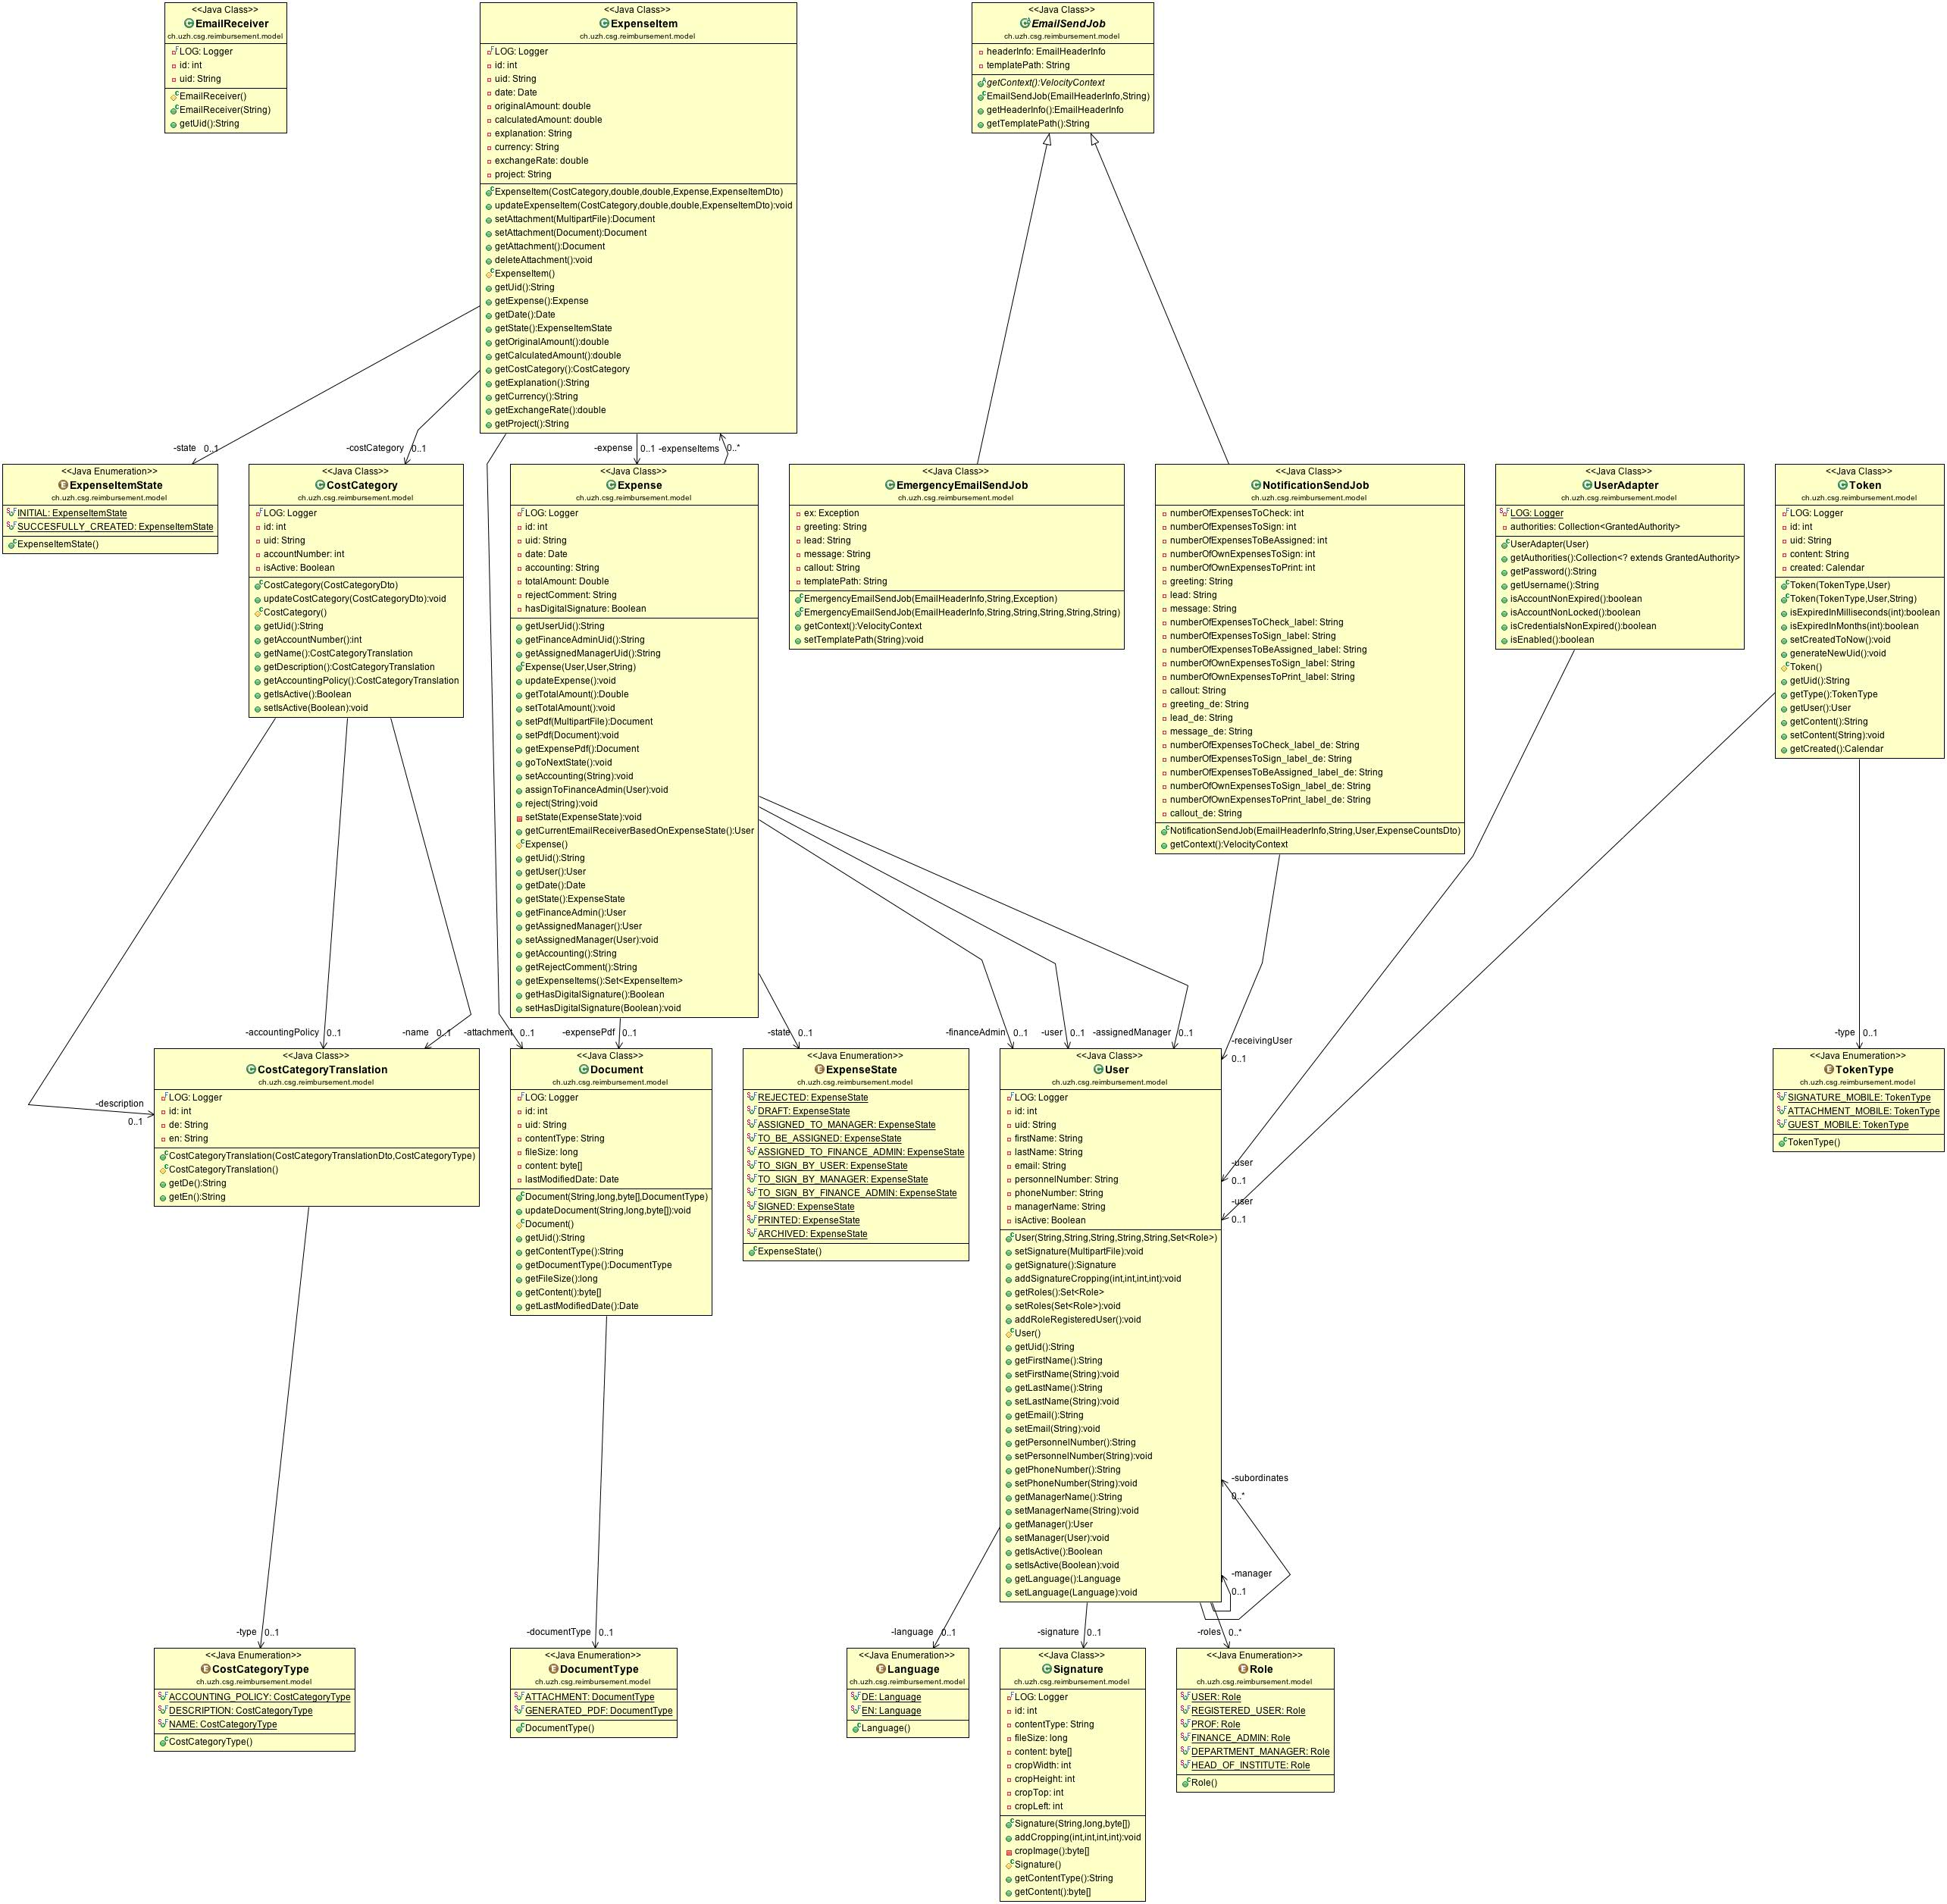
\includegraphics[width=1.0\textwidth]{umlclass-model}}
\end{figure}

\section{Services}
\label{sec:app-service}

\begin{figure}[H]
    {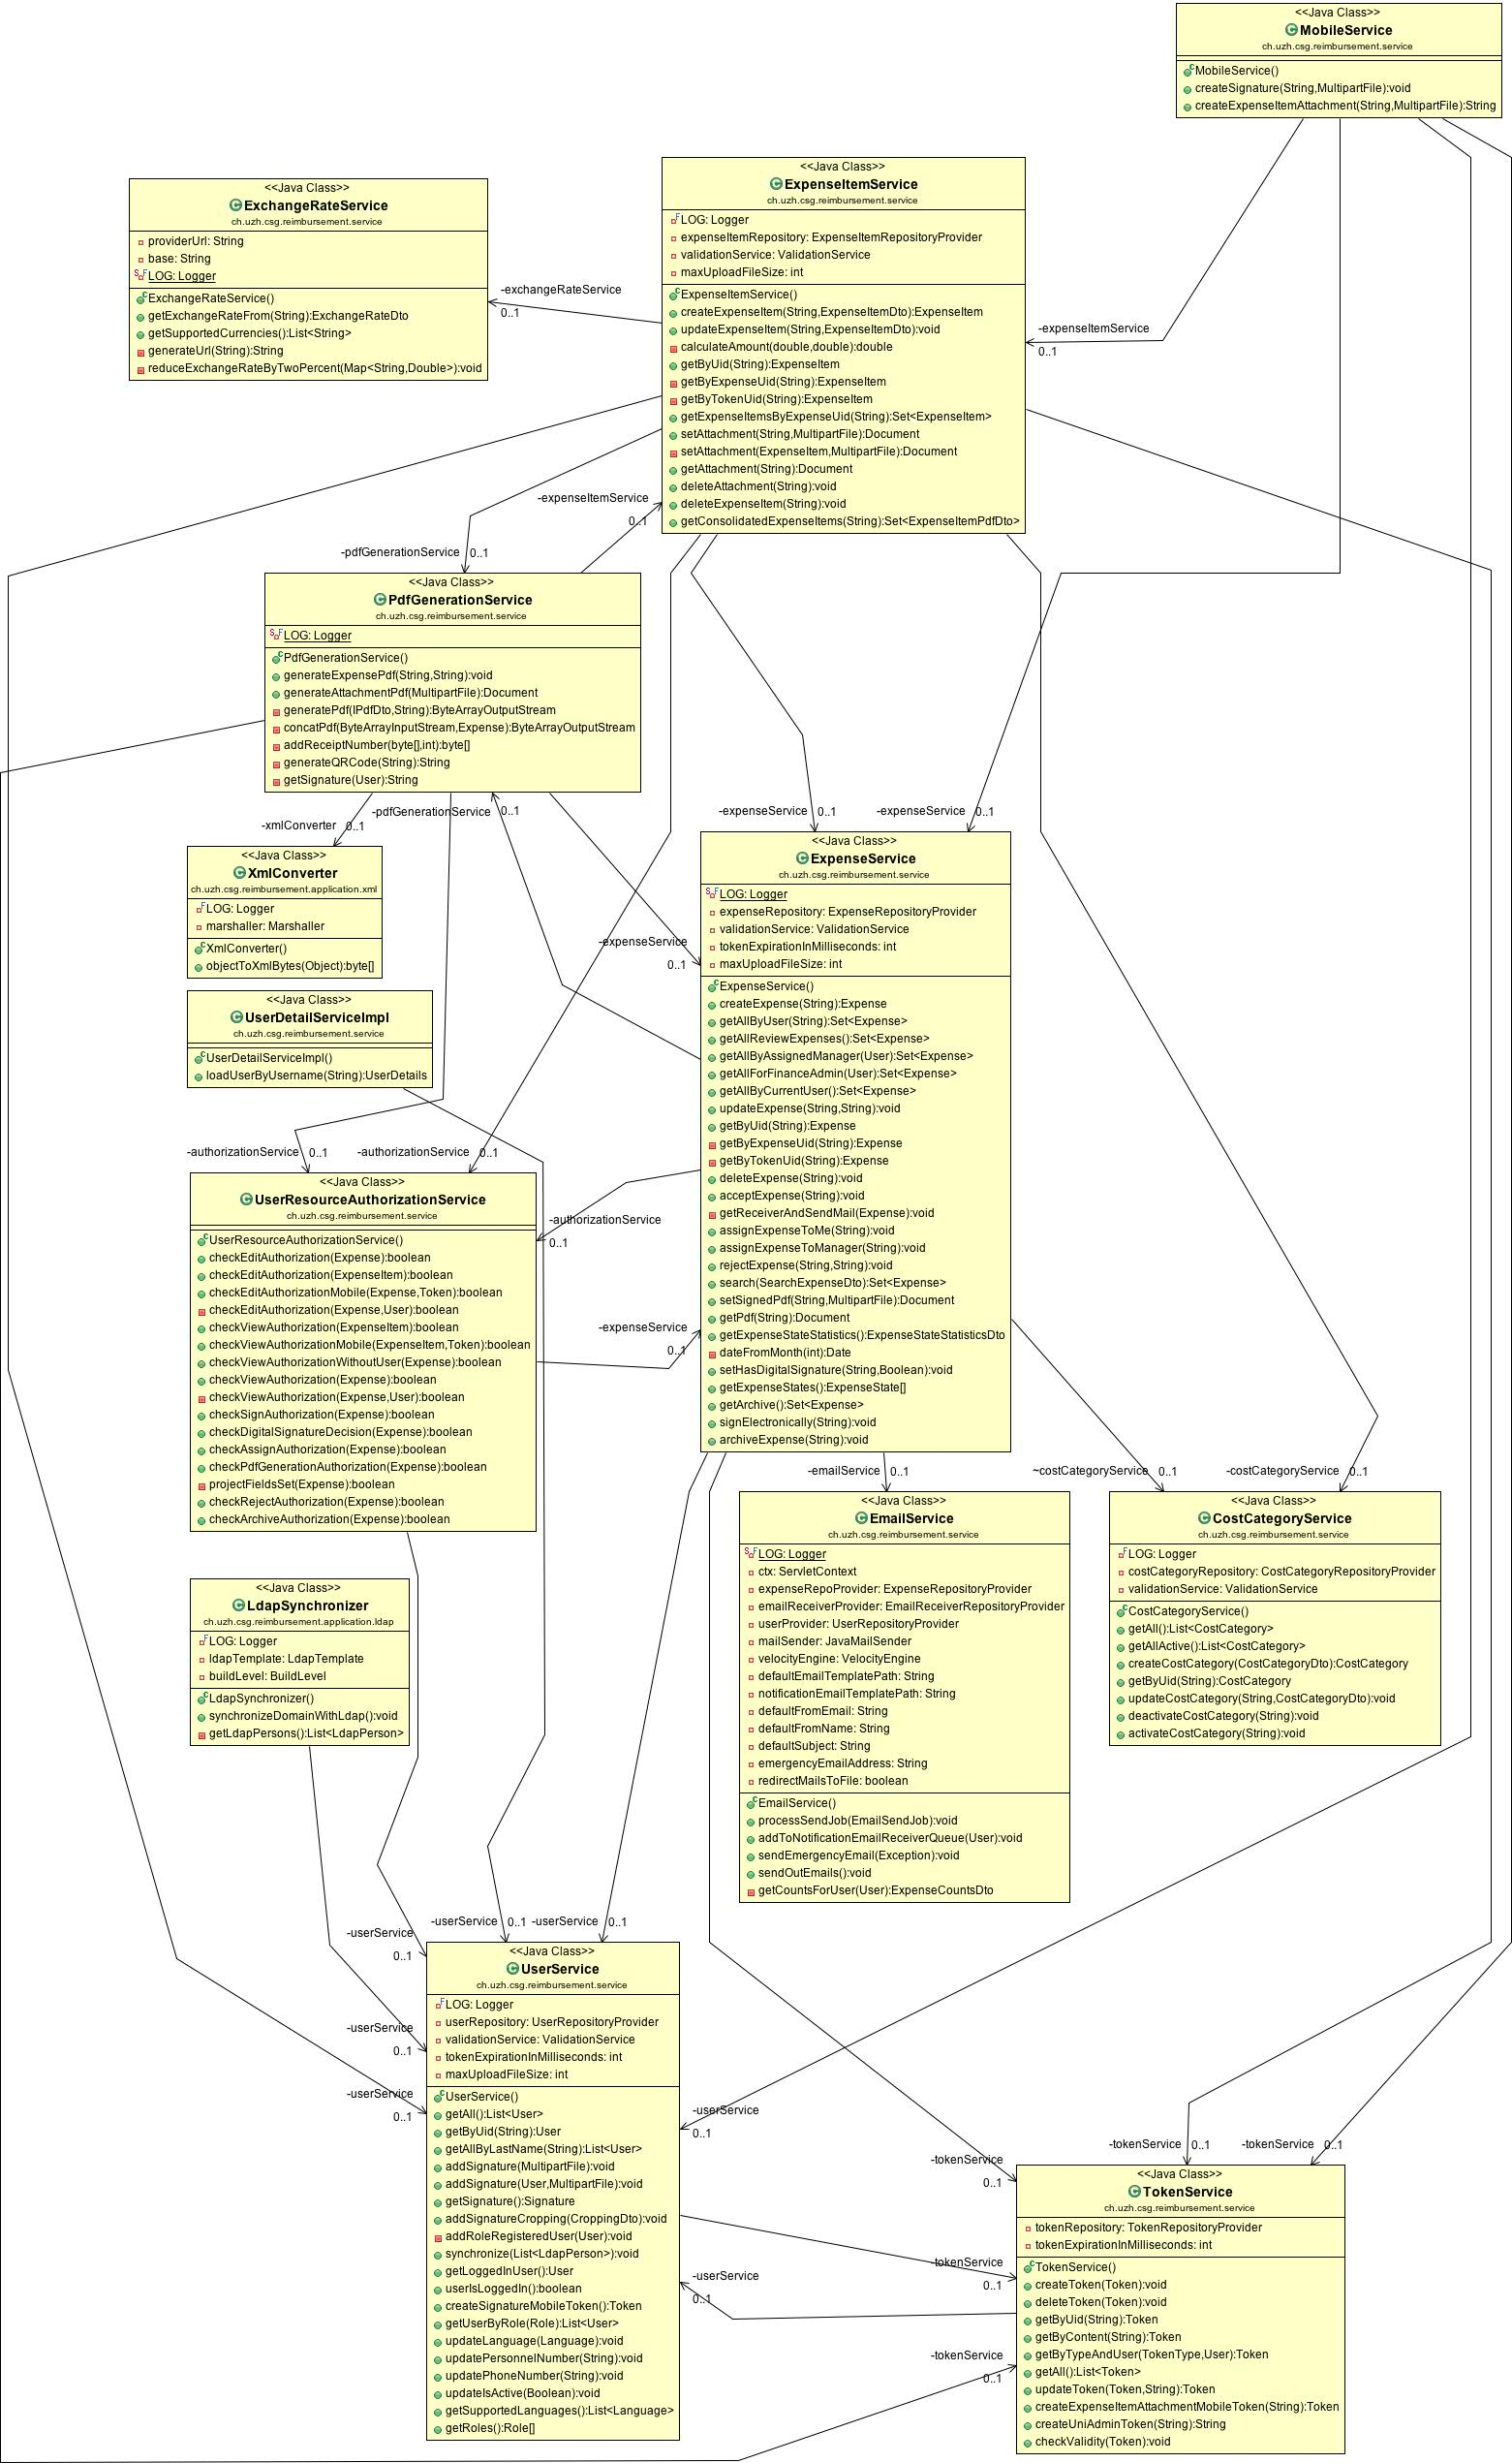
\includegraphics[width=0.95\textwidth]{umlclass-service}}
\end{figure}

\section{Process diagram}
\label{sec:process-diagram-rotated}

\begin{figure}[H]
    {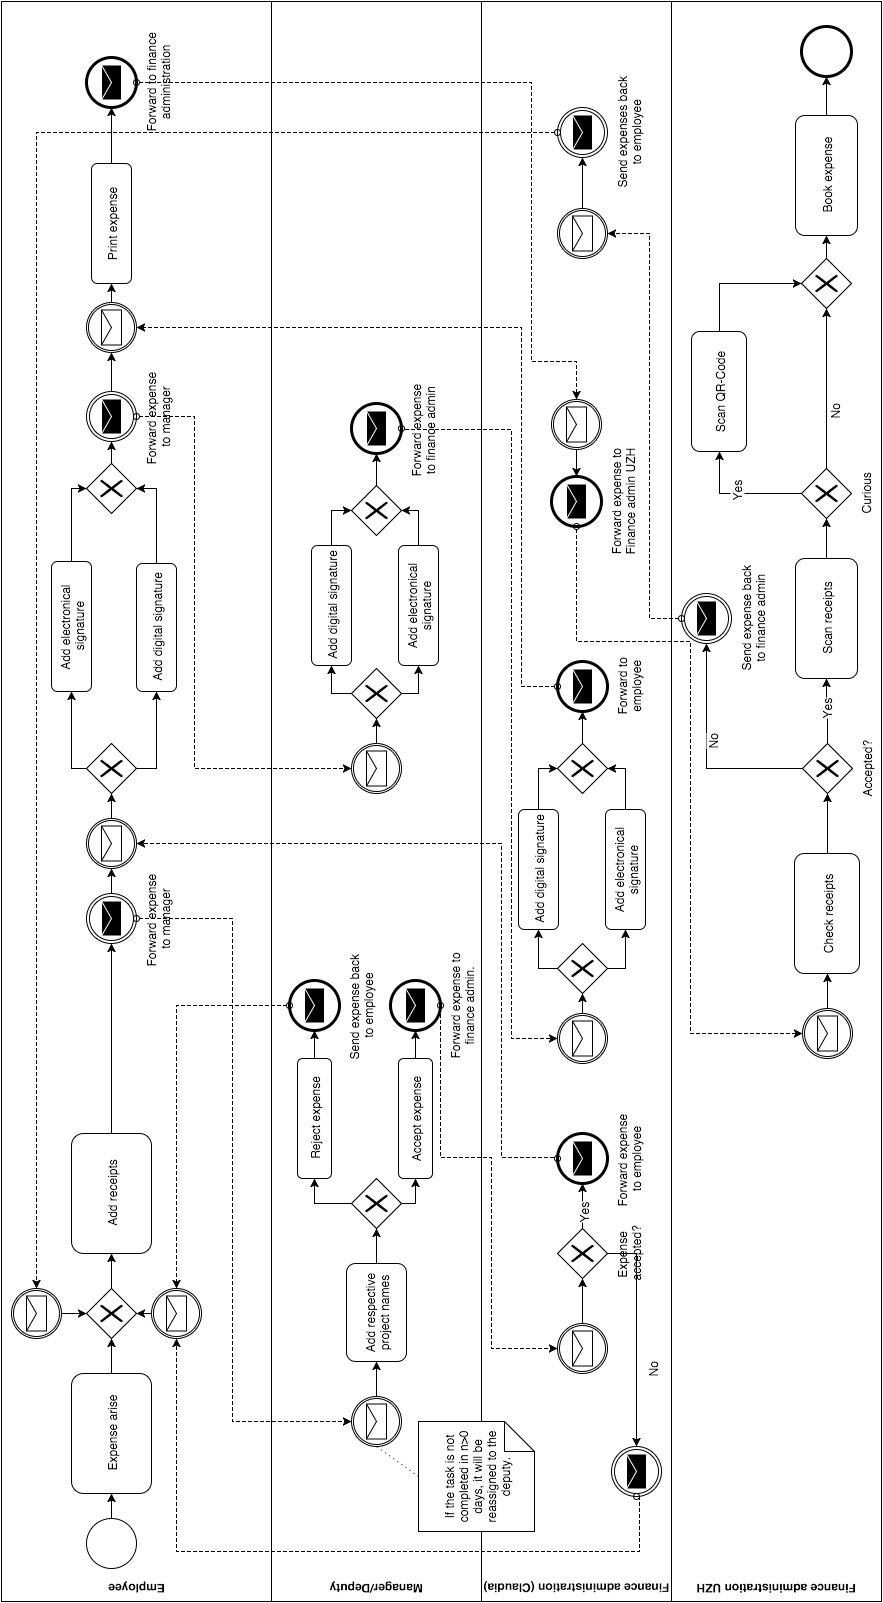
\includegraphics[width=0.8\textwidth]{process-diagram-rotated}}
\end{figure}

\section{State diagram}
\label{sec:state-diagram}

\begin{figure}[H]
    {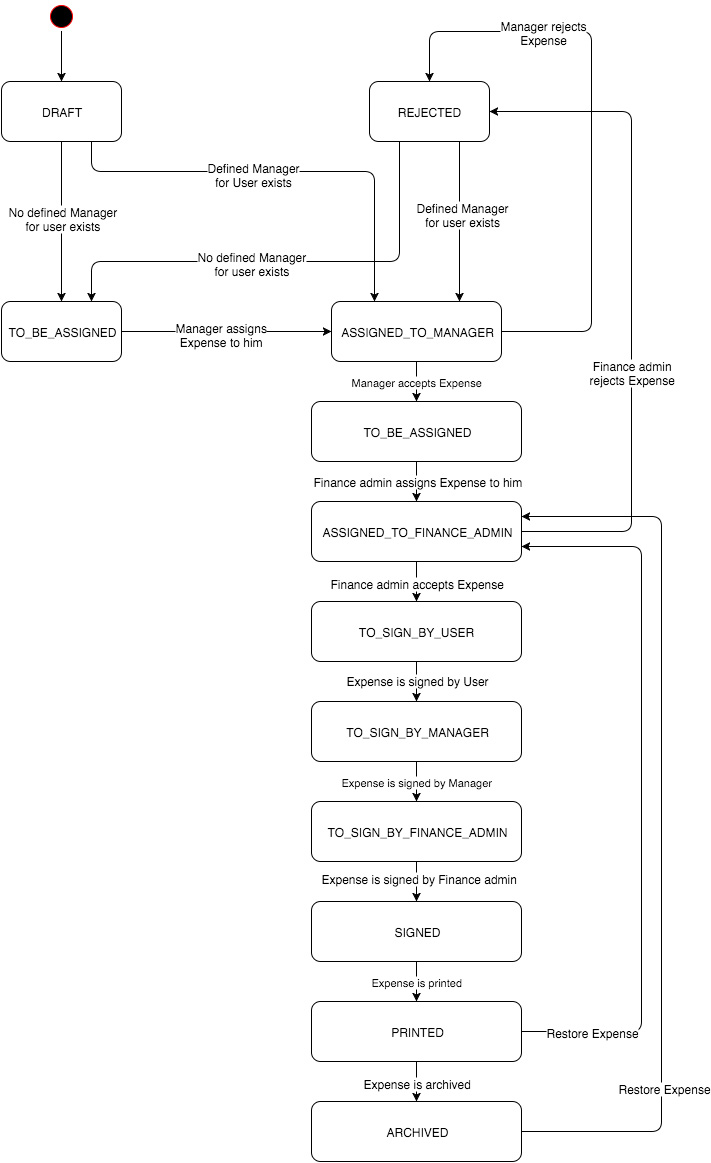
\includegraphics[width=0.8\textwidth]{state-diagram}}
\end{figure}

\section{PDF}
\label{sec:app-pdf}

\begin{figure}[H]
    {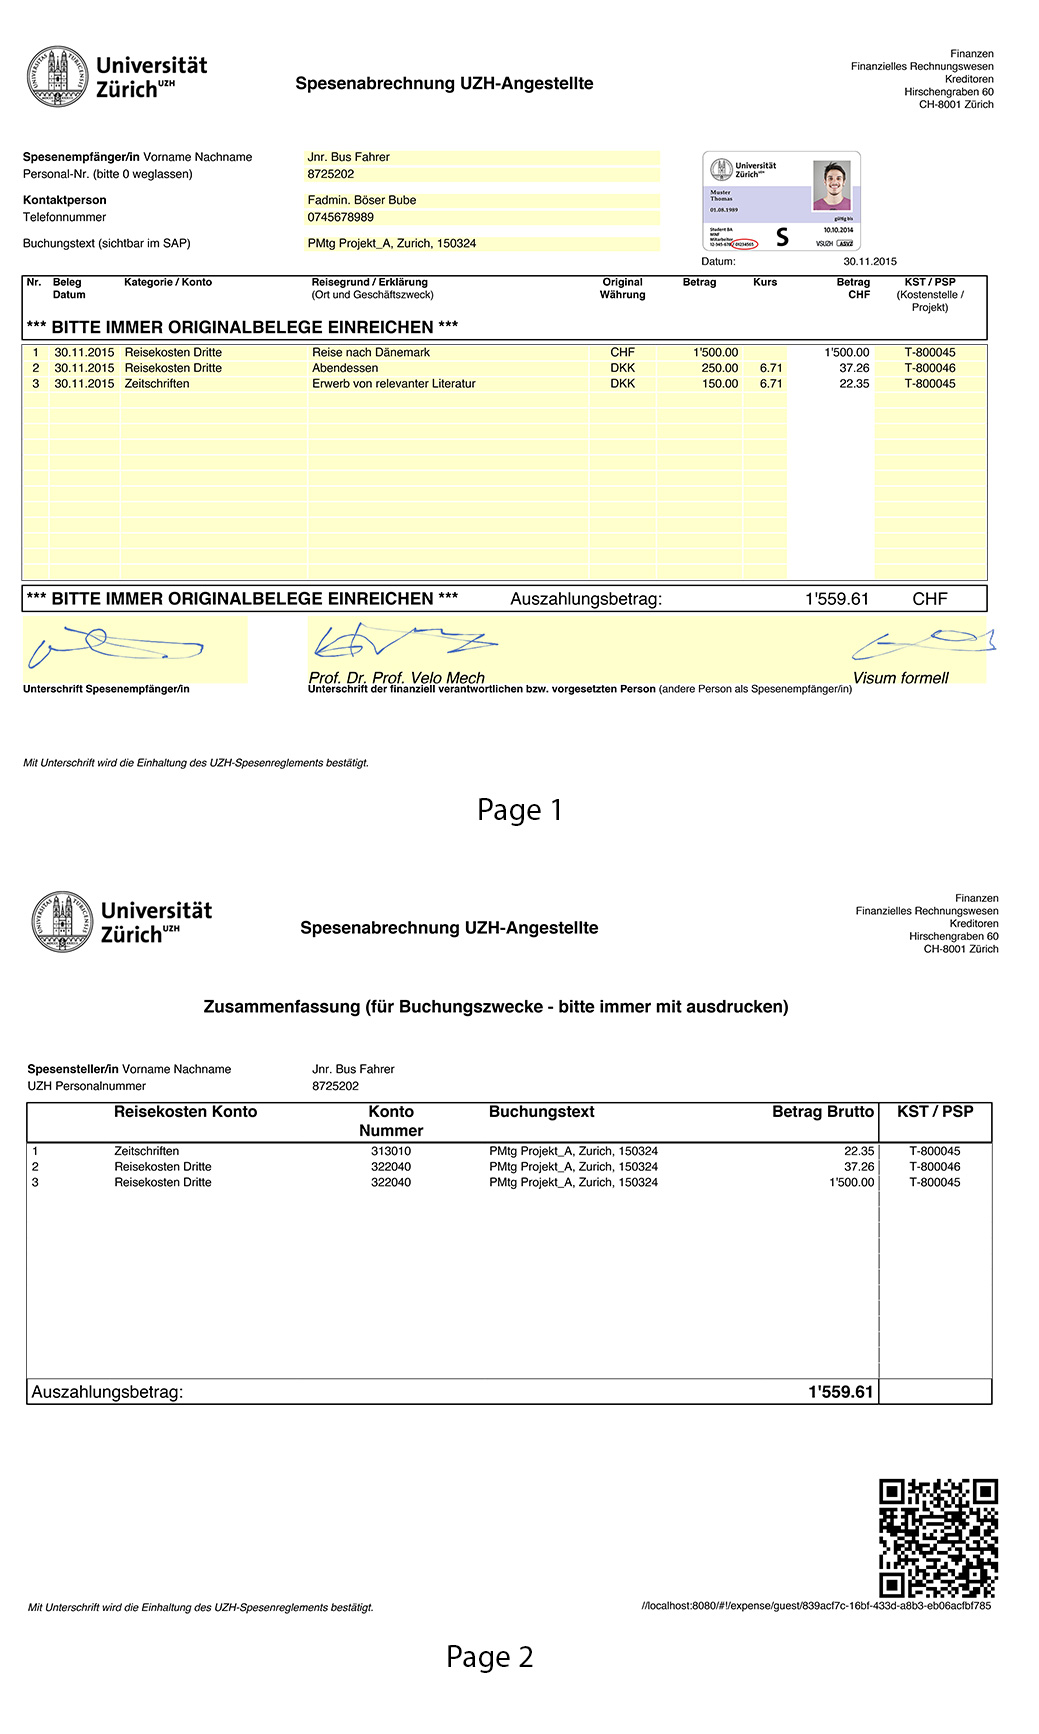
\includegraphics[width=0.95\textwidth]{pdf}}
\end{figure}

\chapter{Software source-code}

The complete software code is available on a public repository on \url{http://github.com}. There exists two repositories; one for the front-end and one for the back-end:

\begin{itemize}
\item Back-end: \newline \url{https://github.com/masterproject-reimbursement/reimbursement-server}
\item Front-end: \newline \url{https://github.com/masterproject-reimbursement/reimbursement-client}
\end{itemize}

For detailed installation instructions, please refer to appendix \ref{chap:installation}. 
